\documentclass[11pt, a4paper]{article}

\usepackage[left=2cm,text={17cm, 24cm},top=3cm]{geometry}
\usepackage{times}
\usepackage[czech]{babel}
\PassOptionsToPackage{hyphens}{url}\usepackage[hidelinks]{hyperref}

\usepackage{graphicx}
\graphicspath{ {./} }

\begin{document}

\begin{titlepage}
    \begin{center}
        \textsc{\Huge Vysoké učení technické v Brně\\\vspace{0.5em}\huge Fakulta informačních technologií}
        
        \vspace{\stretch{0.382}}
        {\LARGE Modelování a simulace -- IMS\\\vspace{0.5em}}
        {\Huge T10: Počítačové služby}
        \vspace{\stretch{0.618}}
        
    \end{center}
    {\Large 2. 12. 2024 \hfill Lukáš Katona, Klára Kejdová}
\end{titlepage}

\newpage

\section{Úvod}

% TODO pociatocna otazka
Cílém této studie je analyzovat sledování příspěvků na sociálních sítích.
Různé skupiny lidí mají různé preference a zájmy, a proto se může stát,
že některé příspěvky nebudou dostatečně sledovány. Cílem je zjistit,
jakým způsobem se šíří informace a jakým způsobem se může zvýšit sledovanost příspěvků.

Poznatky o šíření příspěvků mohou být využity pro zlepšení marketingových strategií,
ale také pro zlepšení algoritmů sociálních sítí, které rozhodují o tom, které příspěvky budou uživatelům zobrazovány.
% TODO comu cheme dospiet
Chtěli bychom zjistit jaké příspěvky jsou relevantí pro různé věkové skupiny.
Co chceme sledovat:
\begin{itemize}
    \item Kolik lidí dokouká příspěvek do konce
    \begin{itemize}
        \item Různé věkové kategorie idí mají jinou dobu pozornosti, proto délka příspěvku hraje roli v tom, jak je daný příspěvěk sledován.
        \item Optimalizací délky příspěšku můžeme zvýšit sledovanost.
    \end{itemize}
    \item Jaká je optimální délka příspěvu pro různé věkové skupiny
    \begin{itemize}
        \item V případě že uživatel nedokouká až do konce, pak nás zajímá, kolik procent příspěvku dokouká.
        \item Nejdůležitější informace by měly být na začátku příspěvku, aby je vidělo co nejvíce uživatelů.
    \end{itemize}
    \item Kolikrát uživatel vidí ten stejný příspěvek
    \begin{itemize}
        \item Pokud uživatel vidí daný příspěvek málokrát a jedná se o reklamu, pak na ni nemusí reagovat.
        \item Přílišené opakování příspěvku však může vést k opačenému efektu, tedy k opětovanému ignorování příspěvku.
    \end{itemize}
    \item Čas zveřejnění příspěvku 
    \begin{itemize}
        \item Čas zveřejnění v různé doby dne může mít vliv na sledovanost příspěvku.
        \item Pokud je příspěvek zveřejněn v době, kdy je uživatel online, pak je pravděpodobnější, že ho uvidí.
    \end{itemize}
\end{itemize}
% TODO k comu sme dospeli
% ako sme vysledky overovali

\section{Fakta}

\subsection{Čas zveřejnění}
Dle \cite{TimeToPost}, jsme zjistili, že nejlepší čas na publikování příspěvků je zhruba mezi 9:00 - 12:00. Zde záleží na sociální síti, 
pro zjednodušení simulace budeme však používat průměrné hodnoty těchto časů.
Tento čas zároveň koreluje s naší vlastní zkušeností, kdy většina lidí bývá online.

\subsection{Délka příspěvku}
Délka příspěvku by měla záviset na schopnpsti lidí udržet pozornost. Záleží na co tito lidé upínají svoji pozornost,
naříklad, na práci se lidé soustředí déle než na sociální sítě, proto bylo náročené najít jednoznačné a konkrétní číslo.
Proto jsme hledali na více zdrojích a tato čísla zprůměrovali na základě našich vlastních zkušeností.

Podle \cite{AttentionSpan1}, starší lidé, přibližně nad 50 roků, mají průměrnou dobu pozornosti 2,5 minuty, zatímco lidé v produktivním věku mají pozornost již sníženou, a to na 40-75 sekund.
Na základě výzkumu \cite{AttentionSpan2}, mají děti pozornost ještě nižší, pouze 2-8 sekund.

\subsection{Opakování příspěvku a jejich sledovanost}
Tento bod je primárně důležitý z hleidska marketingu, aby se nestalo, že se reklamy stanou příliš otravnými.
Podle statustik \cite{SocialMediaAds}, pokud uživatel viděl danou reklamu 11krát a vícekrát, pak je o 10\% pravděpodobnější že na ni bude regovat negativně.
Navíc, pouze 44\% uživatelů dle \cite{SocialMediaAds-44} vidí nerelevantí reklamy. 

Je proto dlůežité, si dát pozor, jak často se budou příspěvky opakovat, aby nebyly otravné, ale zároveň aby byly dostatečně viděny.



% čas zveřejění - kdy je nelepší zveřejnit příspěvek - čas a den
% attention span - jaké věkové kategorie lidí mají jakou dobu pozornosti
% jaká je pravděpodobnost že uživatel sdíli - engagement rate (share, like,...) 
% TODO aspon dva zdroje

\subsection{Hypotézy}
\begin{enumerate}
    \item Délka příspěvku ovlivňuje sledovanost
    \item Čas zveřejnění příspěvku ovlivňuje sledovanost
    \item To, kolikrát uživatel vidí příspěvek, ovlivňuje reakci na něj
    \item Věková kategorie ovlivňuje sledovanost příspěvku
\end{enumerate}

\section{Koncepce, způsob řešení}

\vspace{1em}
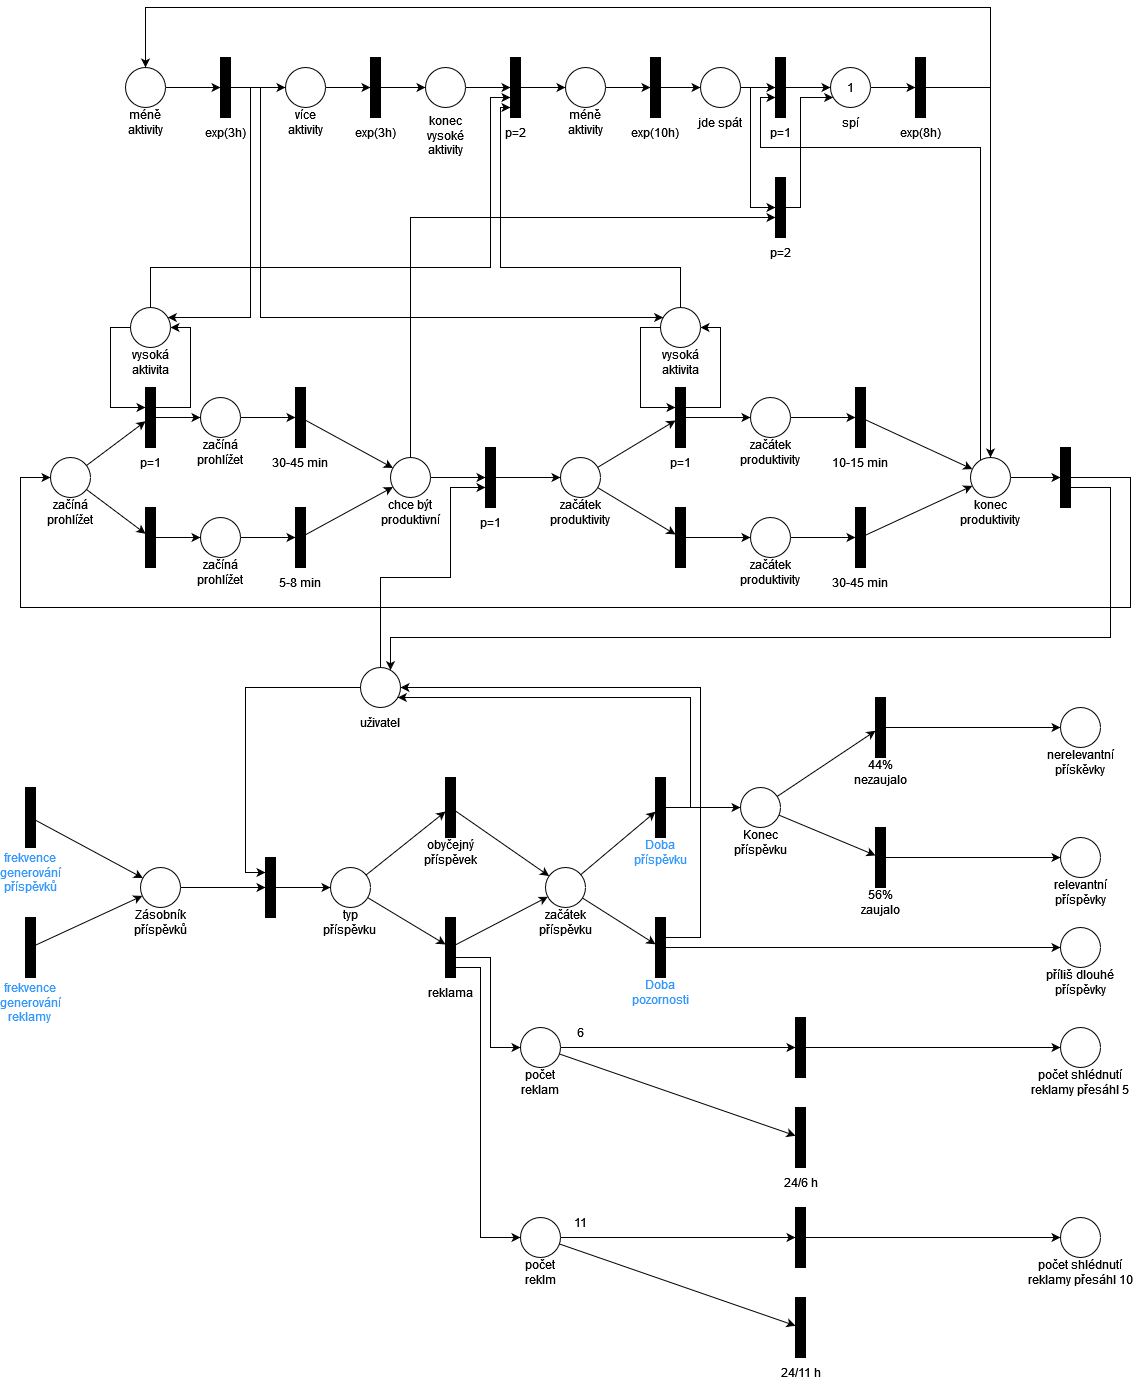
\includegraphics[width=\linewidth]{petri-net.png}
\vspace{1em}

\section{Testování, experimenty}

\section{Závěr}

\bibliographystyle{czechiso}
\bibliography{reference}
    
\end{document}